\section{Divide \& Conquer}

In this approach, first, the input array is divided into 
two halves. Let's call them the left subarray and the 
right subarray, and then we solve those smaller instance 
problems. All possible subarrays are in the left subarray, 
right subarray, or there is another case that the subarray 
crosses the midpoint, in this situation we need to solve 
the problem directly with another help function. You can 
see different scenarios in \textbf{Figure \ref{fig:divide}}. 

\begin{figure}[H]
    \centering
    
\begin{tabular}{cc}
   \subfloat[]{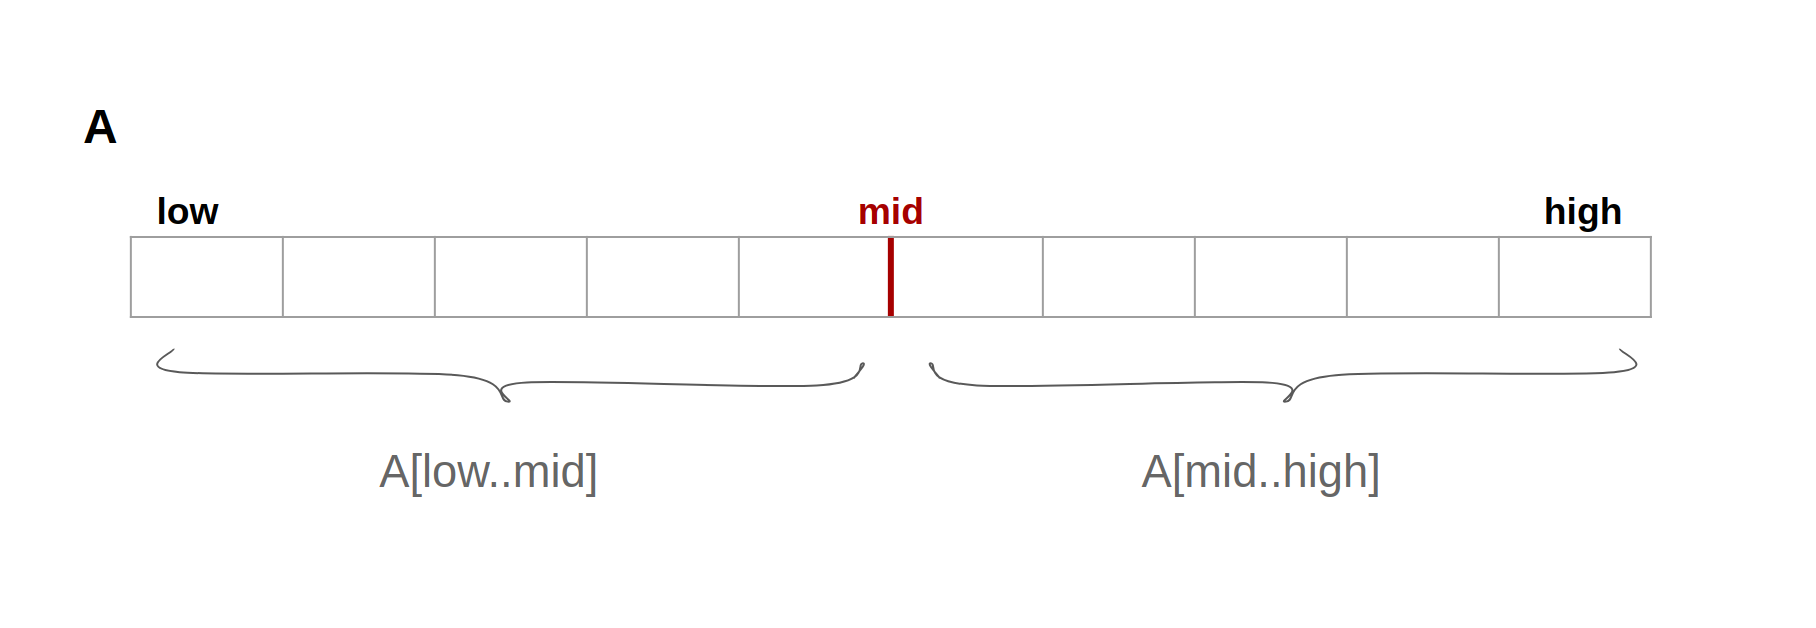
\includegraphics[width = 0.5\textwidth]{images/array_divide.png}} &
\subfloat[]{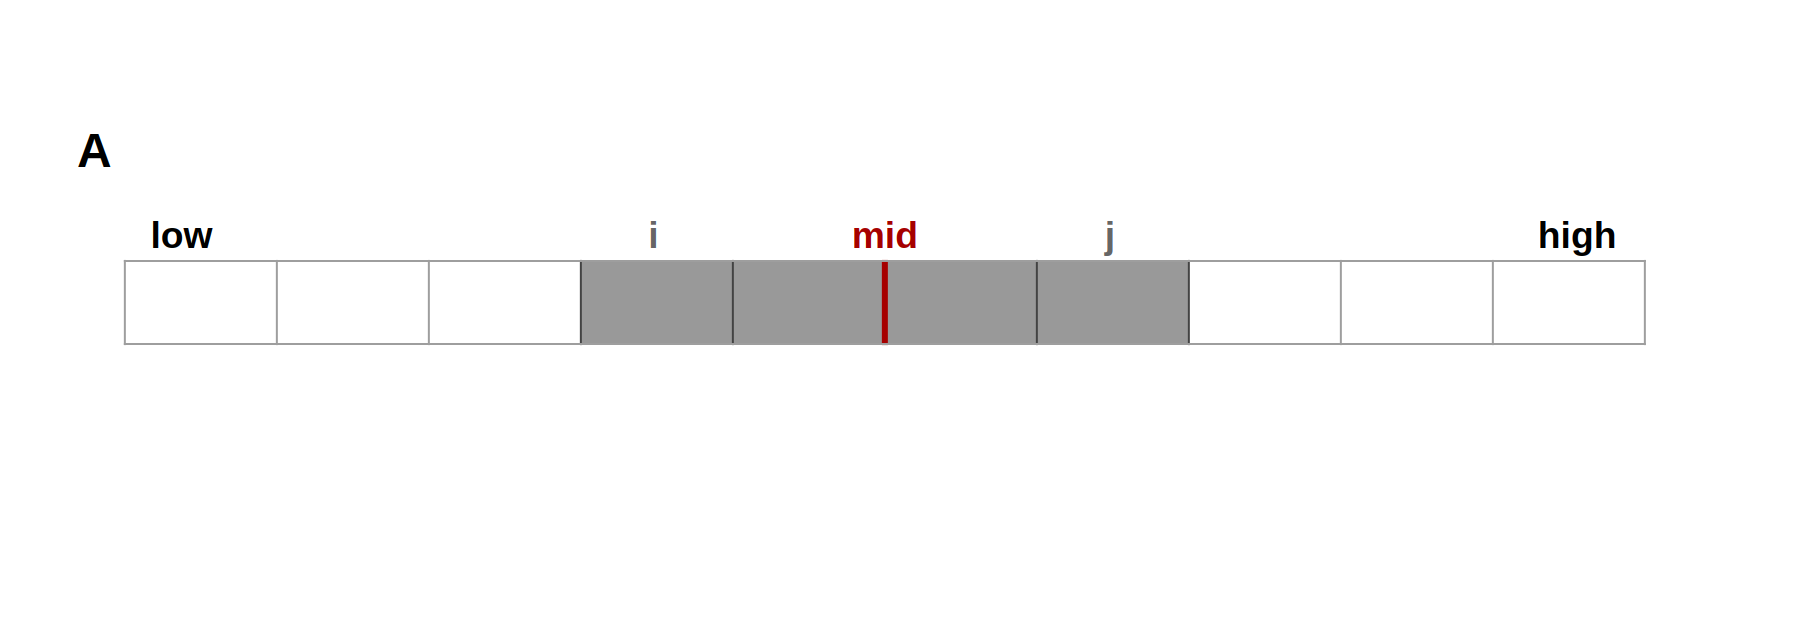
\includegraphics[width = 0.5\textwidth]{images/mid_cross.png}} 
\end{tabular}
    \caption{(a) possible locations of subarrays of A[low..high]: entirely
    in A[low..mid], entirely in A[mid+1..high], (b) or crossing mid. }
    \label{fig:divide}
\end{figure}
First, a function is written to solve the situation that the sub-array 
crosses the middle. The logic is simple, first, start from the middle 
and go to the beginning to find the index \textbf{i} that has the largest 
sum and then do the same thing for the right sub-array, start from the 
middle to the end of the array and store the index \textbf{j} that 
has the maximum value. Then the index and the maximum sum will be returned.
The code is shown in the Listing \ref{list:cross}
\pythonexternal[caption={\textbf{Find the subarray that has the largest value and crosses the middle}},
    label={list:cross}]{codes/find_max_crossing_subarray.py}

The divide-and-conquer form is shown in Listing 
\ref{list:divide}. First, the array is divided into two 
sections. Then the subproblems are solved 
recursively, and their values compare to each 
other to return the one that has the largest value.
\pythonexternal[caption={\textbf{Maximum subarray code using divide and conquer}},
    label={list:divide}]{codes/devide_and_conquer.py}
\subsection{Cost Analysis}
As you can see in the base case, it takes 
$\Theta(1)$ to return the answer. In the 
recursive steps, the problem is divided into 
two subproblems with half the size of the 
original one, so if the run time be $T(n)$, 
then each of them takes $T(\frac{n}{2})$. For 
finding maximum subarray that crosses the 
middle takes $\Theta(n)$ cause we need to 
traverse the whole array once and check if 
the sum is larger than our temp\_max or not
( takes $\Theta(1)$ ).
\[
    T(n)=\begin{cases}
        \Theta(1) & n=1\\
        \Theta(n) + T(\frac{n}{2}) & n \geq 1
    \end{cases}
    \]
Using \textbf{Master Theorem}, it gives $T(n) = \Theta(n\log(n))$.